%%%%%%%%%%%%%%%%%%%%%%%%%%%%%%%%%%%%%%%%%
% Beamer Presentation
% LaTeX Template
% Version 1.0 (10/11/12)
%
% This template has been downloaded from:
% http://www.LaTeXTemplates.com
%
% License:
% CC BY-NC-SA 3.0 (http://creativecommons.org/licenses/by-nc-sa/3.0/)
%
%%%%%%%%%%%%%%%%%%%%%%%%%%%%%%%%%%%%%%%%%

%----------------------------------------------------------------------------------------
%	PACKAGES AND THEMES
%----------------------------------------------------------------------------------------

\documentclass{beamer}

\mode<presentation> {

% The Beamer class comes with a number of default slide themes
% which change the colors and layouts of slides. Below this is a list
% of all the themes, uncomment each in turn to see what they look like.

%\usetheme{default}
%\usetheme{AnnArbor}
%\usetheme{Antibes}
%\usetheme{Bergen}
%\usetheme{Berkeley}
%\usetheme{Berlin}
%\usetheme{Boadilla}
%\usetheme{CambridgeUS}
%\usetheme{Copenhagen}
%\usetheme{Darmstadt}
%\usetheme{Dresden}
%\usetheme{Frankfurt}
%\usetheme{Goettingen}
%\usetheme{Hannover}
%\usetheme{Ilmenau}
%\usetheme{JuanLesPins}
%\usetheme{Luebeck}
\usetheme{Madrid}
%\usetheme{Malmoe}
%\usetheme{Marburg}
%\usetheme{Montpellier}
%\usetheme{PaloAlto}
%\usetheme{Pittsburgh}
%\usetheme{Rochester}
%\usetheme{Singapore}
%\usetheme{Szeged}
%\usetheme{Warsaw}

% As well as themes, the Beamer class has a number of color themes
% for any slide theme. Uncomment each of these in turn to see how it
% changes the colors of your current slide theme.

%\usecolortheme{albatross}
%\usecolortheme{beaver}
%\usecolortheme{beetle}
%\usecolortheme{crane}
%\usecolortheme{dolphin}
%\usecolortheme{dove}
%\usecolortheme{fly}
%\usecolortheme{lily}
%\usecolortheme{orchid}
%\usecolortheme{rose}
%\usecolortheme{seagull}
%\usecolortheme{seahorse}
%\usecolortheme{whale}
%\usecolortheme{wolverine}

%\setbeamertemplate{footline} % To remove the footer line in all slides uncomment this line
%\setbeamertemplate{footline}[page number] % To replace the footer line in all slides with a simple slide count uncomment this line

%\setbeamertemplate{navigation symbols}{} % To remove the navigation symbols from the bottom of all slides uncomment this line
}

\usepackage{graphicx} % Allows including images
% \usepackage{booktabs} % Allows the use of \toprule, \midrule and \bottomrule in tables
\usepackage{lmodern}
% \usepackage{verbatim}
% \usepackage{tabto}
% \usepackage{listings}
% \usepackage{mathtools}
% \usepackage{amsmath}
% \usepackage{makecell}
\usepackage{tikz}
\usepackage{pifont}
\usepackage[utf8]{inputenc}
\usepackage{subcaption}
\usepackage{multirow}

% \newcommand*\m[1]{
% 	\tikz[baseline=(char.center)]{
%     	\node[shape=circle,draw,inner sep=0.3pt] (char) {#1}
% 	}
% }
\def\m#1{{\normalsize\textcircled{\scriptsize #1}}}
\def\code#1{\texttt{#1}}

\newcommand\blfootnote[1]{%
	\scriptsize
	\begingroup
	\renewcommand\thefootnote{}\footnote{#1}%
	\addtocounter{footnote}{-1}%
	\endgroup
}
\newcommand\safepi[0]{
	\texorpdfstring{$\pi$}{Pi}
}


%----------------------------------------------------------------------------------------
%	TITLE PAGE
%----------------------------------------------------------------------------------------

% The short title appears at the bottom of every slide, the full title is only on the title page
\title[Sistemas Operacionais]{Sistemas Operacionais} 

\author{Bruno Feitosa} % Your name
\institute[USP] % Your institution as it will appear on the bottom of every slide, may be shorthand to save space
{
Universidade de São Paulo \\ % Your institution for the title page
\medskip
\textit{feitosa.bruno@usp.com} % Your email address
}
\date{24/06/2019} % Date, can be changed to a custom date

\begin{document}
\setbeamertemplate{caption}{\raggedright\insertcaption\par}

%------------------------------------------------------------------------------

\begin{frame}

\titlepage % Print the title page as the first slide

\end{frame}

%------------------------------------------------------------------------------

\begin{frame}

\frametitle{Resumo} % Table of contents slide, comment this block out to remove it
\tableofcontents % Throughout your presentation, if you choose to use \section{} and \subsection{} commands, these will automatically be printed on this slide as an overview of your presentation

\end{frame}

%------------------------------------------------------------------------------

%------------------------------------------------------------------------------
%	PRESENTATION SLIDES
%------------------------------------------------------------------------------

%------------------------------------------------------------------------------

\begin{frame}

\section{Cálculo do \safepi}
\frametitle{Cálculo do \safepi}

\begin{itemize}
    \item Gauss-Legendre
    \item BBP
    \item Monte Carlo
\end{itemize}

\end{frame}

%------------------------------------------------------------------------------

\begin{frame}

\subsection{Método Gauss-Legendre}
\frametitle{Cálculo do \safepi: Gauss-Legendre}

\begin{itemize}
    \item Aplicação da regra de quadratura Gauss-Legendre
    \item Rápida Convergência, porém, Alto Custo
\end{itemize}

\begin{equation}
	\begin{aligned}
		a_{n+1} &= \frac{a_n + b_n}{2}			& a_0 &= 1\\
		b_{n+1} &= \sqrt{a_n b_n}				& b_0 &= \frac{1}{\sqrt{2}} \\
		t_{n+1} &= t_n - p_n(a_{n}-a_{n+1})^2	& t_0 &= \frac{1}{4} \\
		p_{n+1} &= 2p_n							& p_0 &= 1		
	\end{aligned}
\end{equation}
\begin{equation}
	\pi \approx \frac{(a_{n+1}+b_{n+1})^2}{4.t_{n+1}}
\end{equation}
	
\end{frame}

%------------------------------------------------------------------------------

\begin{frame}

\frametitle{Cálculo do \safepi: Gauss-Legendre}

\scriptsize
\renewcommand*{\arraystretch}{1.3}
\begin{table}[h]
	\centering
	\begin{tabular}{|l|c|c|c|c|c|}
		\hline
		$n$ & $a_n$	& $b_n$ & $t_n$ & $p_n$ & $(a_n - b_n)$\\ 
		\hline
		0& 1.000000e+00& 7.071068e-01& 2.500000e-01& 1.000000e+00& 2.928932e-01\\
		1& 8.535534e-01& 8.408964e-01& 2.285534e-01& 2.000000e+00& 1.265698e-02\\
		2& 8.472249e-01& 8.472013e-01& 2.284733e-01& 4.000000e+00& 2.363618e-05\\
		3& 8.472131e-01& 8.472131e-01& 2.284733e-01& 8.000000e+00& 8.242744e-11\\
		4& 8.472131e-01& 8.472131e-01& 2.284733e-01& 1.600000e+01& 1.002446e-21\\
		5& 8.472131e-01& 8.472131e-01& 2.284733e-01& 3.200000e+01& 1.482652e-43\\
		6& 8.472131e-01& 8.472131e-01& 2.284733e-01& 6.400000e+01& 3.243366e-87\\
		7& 8.472131e-01& 8.472131e-01& 2.284733e-01& 1.280000e+02& 1.552063e-174\\
		8& 8.472131e-01& 8.472131e-01& 2.284733e-01& 2.560000e+02& 3.554152e-349\\
		9& 8.472131e-01& 8.472131e-01& 2.284733e-01& 5.120000e+02& 1.863758e-698\\
	   10& 8.472131e-01& 8.472131e-01& 2.284733e-01& 1.024000e+03& 5.125029e-1397\\
	   \hline
	\end{tabular}
\end{table}
\renewcommand*{\arraystretch}{1}
\normalsize
	
\end{frame}

%------------------------------------------------------------------------------

\begin{frame}

\frametitle{Cálculo do \safepi: Gauss-Legendre}

\scriptsize
\renewcommand*{\arraystretch}{1.3}
\begin{table}[h]
	\centering
	\begin{tabular}{|l|c|}
		\hline
		$n$ & $\pi$\\ 
		\hline
		0& 2.91421356237309504880168872420969807856967187537695\\
		1& 3.14057925052216824831133126897582331177344023751295\\
		2& 3.14159264621354228214934443198269577431443722334560\\
		3& 3.14159265358979323827951277480186397438122550483545\\
		4& 3.14159265358979323846264338327950288419711467828365\\
		5& 3.14159265358979323846264338327950288419716939937511\\
		6& 3.14159265358979323846264338327950288419716939937511\\
		7& 3.14159265358979323846264338327950288419716939937511\\
		8& 3.14159265358979323846264338327950288419716939937511\\
		9& 3.14159265358979323846264338327950288419716939937511\\
	   10& 3.14159265358979323846264338327950288419716939937511\\			   
	   \hline
	   ref& 3.14159265358979323846264338327950288419716939937511\\
	   \hline
	\end{tabular}
\end{table}
\renewcommand*{\arraystretch}{1}
\normalsize
	
\end{frame}

%------------------------------------------------------------------------------

\begin{frame}

\subsection{Método Bailey-Borwein-Plouffe}
\frametitle{Cálculo do \safepi: Bailey-Borwein-Plouffe}

\begin{itemize}
    \item Otimizado para Cálculo Computacional (múltiplos de 8 / byte)
\end{itemize}

\begin{equation}
	\pi \quad = \quad \sum_{k=0}^{\infty}\left(\frac{1}{16^k}\right).
	\left(
		\frac{4}{8.k + 1} - \frac{2}{8.k + 4} - \frac{1}{8.k + 5} - \frac{1}{8.k + 6}
	\right)
\end{equation}

\begin{equation}
	\pi \quad = \quad \sum_{k=0}^{\infty} a_k.
	\left(p^1_k + p^2_k + p^3_k + p^4_k\right)
\end{equation}
		
\end{frame}

%------------------------------------------------------------------------------

\begin{frame}

\frametitle{Cálculo do \safepi: Bailey-Borwein-Plouffe}

\scriptsize
\renewcommand*{\arraystretch}{1.3}
\begin{table}[h]
	\centering
	\begin{tabular}{|l|c|c|c|c|c|}
		\hline
		$k$ & $a_k$	& $p_k^1$ & $p_k^2$ & $p_k^3$ & $p_k^4$\\ 
		\hline
		0& 1.000000e+00& 4.000000e+00& -5.000000e-01& -2.000000e-01& -1.666667e-01\\
		1& 6.250000e-02& 4.444444e-01& -1.666667e-01& -7.692308e-02& -7.142857e-02\\
		2& 3.906250e-03& 2.352941e-01& -1.000000e-01& -4.761905e-02& -4.545455e-02\\
		3& 2.441406e-04& 1.600000e-01& -7.142857e-02& -3.448276e-02& -3.333333e-02\\
		4& 1.525879e-05& 1.212121e-01& -5.555556e-02& -2.702703e-02& -2.631579e-02\\
		5& 9.536743e-07& 9.756098e-02& -4.545455e-02& -2.222222e-02& -2.173913e-02\\
		6& 5.960464e-08& 8.163265e-02& -3.846154e-02& -1.886792e-02& -1.851852e-02\\
		7& 3.725290e-09& 7.017544e-02& -3.333333e-02& -1.639344e-02& -1.612903e-02\\
		8& 2.328306e-10& 6.153846e-02& -2.941176e-02& -1.449275e-02& -1.428571e-02\\
		9& 1.455192e-11& 5.479452e-02& -2.631579e-02& -1.298701e-02& -1.282051e-02\\
		\hline
	\end{tabular}
\end{table}
\renewcommand*{\arraystretch}{1}
\normalsize
	
\end{frame}

%------------------------------------------------------------------------------

\begin{frame}

\frametitle{Cálculo do \safepi: Bailey-Borwein-Plouffe}

\scriptsize
\renewcommand*{\arraystretch}{1.3}
\begin{table}[h]
	\centering
	\begin{tabular}{|l|c|}
		\hline
		$k$ & $\pi$\\ 
		\hline
		0& 3.13333333333333333333333333333333333333333333333333\\
		1& 3.14142246642246642246642246642246642246642246642247\\
		2& 3.14158739034658152305211128740540505246387599328776\\
		3& 3.14159245756743538183700455505729339400738995059482\\
		4& 3.14159264546033631955702122244238183172740661797991\\
		5& 3.14159265322808753473437803553620446955852801219780\\
		6& 3.14159265357288082778524076189589848423906560378661\\
		7& 3.14159265358897270494077776717018944697112048981182\\
		8& 3.14159265358975227523617786839810222579502463340906\\
		9& 3.14159265358979114638877696591034741477901588848900\\
	   \hline
	   ref& 3.14159265358979323846264338327950288419716939937511\\
	   \hline
	\end{tabular}
\end{table}
\renewcommand*{\arraystretch}{1}
\normalsize
	
\end{frame}

%------------------------------------------------------------------------------

\begin{frame}

\subsection{Método Monte Carlo}
\frametitle{Cálculo do \safepi: Monte Carlo}
	
\begin{itemize}
    \item Método Estocástico com Convergência Lenta
    \item Cada ponto tem $\pi/4$ chance de cair dentro do circulo
\end{itemize}

\begin{figure}
	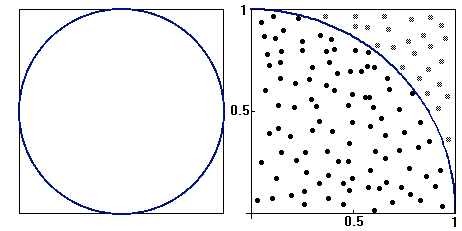
\includegraphics[width=0.8\linewidth]{fig01.png}
\end{figure}
			
\end{frame}

%------------------------------------------------------------------------------

\begin{frame}

\subsection{Comparação dos Métodos}
\frametitle{Comparação dos Métodos}

\small
\begin{itemize}
    \item Gauss-Legendre (GL), Bailey-Borwein-Plouffe (BBP), Monte Carlo (MC)
    \item $15.10^3$ iterações para GL e BBP, $1.10^9$ para MC
    \item 1KB de Precisão para todas variáveis de todos algoritmos
\end{itemize}

\renewcommand*{\arraystretch}{1.3}
\begin{table}[h]
	\centering
	\begin{tabular}{|r|l|c|c|}
		\hline
		\multicolumn{2}{|c|}{Método}	& Não Paralelizado & Paralelizado \\
		\hline
		\multirow{3}{*}{GL} & real 		& 0,229s - 0,235s	& 0,682s - 0,720s \\
							& user 		& 0,229s - 0,235s	& 0,407s - 0,486s \\
							& system	& 0,000s			& 0,300s - 0,371s \\
		\hline
		\multirow{3}{*}{BBP} & real 	& 0,473s - 0,483s	& 1,771s - 1,871s \\
							& user 		& 0,473s - 0,479s	& 1,467s - 1,648s \\
							& system 	& 0,004s - 0,005s	& 2,142s - 2,388s \\
		\hline
		\multirow{3}{*}{MC} & real 		& 7m7,959s	& - \\
							& user 		& 7m7,940s	& - \\
							& system	& 0m0,012s	& - \\
		\hline
	\end{tabular}
\end{table}
\renewcommand*{\arraystretch}{1}
\normalsize

\end{frame}

%------------------------------------------------------------------------------

\begin{frame}

\section{Precificação de Opções}
\frametitle{Precificação de Opções}
	
\begin{itemize}
	\item Opções: Contratos de Compra/Venda com preço fixo
	\item Quem compra o contrato tem o direito de executá-lo
	\item Contrato de Compra: \textit{Call} | Contrato de Venda: \textit{Put}
	\item Preços Envolvidos na Transação:
	\begin{itemize}
		\item Preço da Ação: $P_{\textrm{ação}}$
		\item Preço de Execução: $P_{\textrm{execução}}$
		\item Preço do Contrato: $P_{\textrm{opção}}$
	\end{itemize}
	\item Custo para quem Compra uma \textit{Call} (simplificado sem juros)
	\begin{itemize}
		\item Em caso de Execução: $Custo = P_{\textrm{opção}} + P_{\textrm{execução}}$
		\item Caso Contrário: $Custo = P_{\textrm{opção}}$
	\end{itemize}
	\item Para \textit{Calls}, em geral
	\begin{itemize}
		\item Se $P_{\textrm{execução}} < P_{\textrm{ação}}$, $P_{\textrm{opção}}$ é ``alto''
		\item Se $P_{\textrm{execução}} > P_{\textrm{ação}}$, $P_{\textrm{opção}}$ é ``baixo''
	\end{itemize}
\end{itemize}
	
\end{frame}

%------------------------------------------------------------------------------

\begin{frame}

\subsection{Método de Black Scholes}
\frametitle{Precificação de Opções: Método de Black Scholes}
	
\begin{itemize}
	\item Assume que o Preço da Ação assume uma distribuição normal
	\begin{itemize}
		\item Volatilidade dita o quanto o preço da ação varia
	\end{itemize}
	\item Juros ajustam os preços/custos
	\item O Preço da Opção tenta manter a transação justa (\textit{hedging})
	\item Variáveis:
	\begin{itemize}
		\item $E$: Preço de Execução
		\item $S$: Preço da Ação
		\item $r$: Juros Livre de Risco
		\item $v$: Volatilidade
		\item $T$: Tempo até a Execução
	\end{itemize}
\end{itemize}

\begin{equation}
	\begin{aligned}
		\mathtt{t}			&= S.e^{(r-\frac{v^2}{2}).T}.e^{(v.\sqrt{T}).randomNumber()}\\
		\mathtt{trial[i]}	&= e^{-r.T}.\mathtt{max}(\mathtt{t}-E;0)\\
	\end{aligned}
\end{equation}

\end{frame}

%------------------------------------------------------------------------------

\begin{frame}

\frametitle{Precificação de Opções: Método de Black Scholes}
	
\begin{equation}
	\begin{aligned}
		\mathtt{t}			&= S.e^{(r-\frac{v^2}{2}).T}.e^{(v.\sqrt{T}).randomNumber()}\\
		\mathtt{aux1}		&= S.e^{(r-\frac{v^2}{2}).T}\\
		\mathtt{aux2}		&= (v.\sqrt{T})\\
		\mathtt{trial[i]}	&= e^{-r.T}.\mathtt{max}(\mathtt{t}-E;0)\\
		\mathtt{aux3}		&= e^{-r.T}
	\end{aligned}
\end{equation}
\begin{equation}
	\begin{aligned}
	\mathtt{t}>E \quad &... \quad randomNumber() < \frac{ln(E/\mathtt{aux1})}{\mathtt{aux2}}\\
					   &... \quad randomNumber() < \frac{ln(E/S) - (r-\frac{v^2}{2}).T}{(v.\sqrt{T})}\\
	\end{aligned}
\end{equation}

\end{frame}
	
%------------------------------------------------------------------------------

\begin{frame}
\Huge{\centerline{Fim}}
\end{frame}

%----------------------------------------------------------------------------------------

\end{document}